\documentclass[
	xcolor=dvipsnames,
%	handout
]{beamer}

\usetheme{zhaw}

\usepackage{nameref}
\usepackage{amssymb}
\usepackage{amsmath}

\usepackage[utf8]{inputenc}
\usepackage[T1]{fontenc}

\usepackage{tabularx,colortbl}
\usepackage{xcolor}
\usepackage{listings}
\usepackage{upquote}
\usepackage{url}
\usepackage{etoolbox}
\usepackage{graphicx}
\usepackage{synttree}
\usepackage{listings}
\usepackage{multicol}

\definecolor{gray_ulisses}{gray}{0.55}
\definecolor{castanho_ulisses}{rgb}{0.71,0.33,0.14}
\definecolor{preto_ulisses}{rgb}{0.41,0.20,0.04}
\definecolor{green_ulises}{rgb}{0.2,0.75,0}

\definecolor{background}{RGB}{240, 240, 190}
\definecolor{string}{RGB}{230, 219, 116}
\definecolor{comment}{RGB}{117, 113, 94}
\definecolor{normal}{RGB}{248, 248, 242}
\definecolor{identifier}{RGB}{166, 226, 46}

\lstdefinelanguage{Golang}{
	morekeywords=[1]{package,import,func,type,struct,return,defer,panic,recover,select,var,const,iota},
	morekeywords=[2]{string,uint,uint8,uint16,uint32,uint64,int,int8,int16,int32,int64,bool,float32,float64,complex64,complex128,byte,rune,uintptr,error,interface},
	morekeywords=[3]{map,slice,make,new,nil,len,cap,copy,close,true,false,delete,append,real,imag,complex,chan},
	morekeywords=[4]{for,break,continue,range,go,goto,switch,case,fallthrough,if,else,default},
	morekeywords=[5]{Println,Printf,Error,Print},
	sensitive=true,
	morecomment=[l]{//},
	morecomment=[s]{/*}{*/},
	morestring=[b]',
	morestring=[b]",
	morestring=[s]{`}{`},
}
\lstdefinestyle{basestyle}{
	basicstyle=\small\ttfamily,
	breakatwhitespace = true,
	tabsize = 4,
	frame = double,
%	numbers = left,
	numbersep = 10pt,
%	numberstyle = {\tiny\emptyaccsupp},
%	firstnumber = auto,
	numberblanklines = true,
	captionpos = b,
	columns = fullflexible,
	extendedchars = true,
	float = ht,
	showtabs = false,
	showspaces=false,
	showstringspaces=false,
	breaklines=true,
%	prebreak=\Righttorque
	backgroundcolor=\color{background!40!white},
	keywordstyle=\color{blue!70!castanho_ulisses}\bfseries,
	commentstyle=\color{green!50!castanho_ulisses}\ttfamily,
%	morekeywords={printstr, printhexln},
	stringstyle=\color{red!70!castanho_ulisses},
	xleftmargin = \fboxsep,
	xrightmargin = -6pt,
	showstringspaces=true,
}

\newenvironment{zhawframe}[1][]
{\begin{frame}[environment=fr,#1]{\insertsectionhead}{\insertsubsectionhead}}
{\end{frame}
}

\setbeamertemplate{footline}[frame number]

\title{Design and Implementation of an Alternative to SSH}
\date{\today}
\author{Raphael Emberger}

\begin{document}
\maketitle

\section*{Index}
\begin{zhawframe}[shrink]
\begin{multicols}{2}
\tableofcontents
\end{multicols}
\end{zhawframe}

\section{Introduction}
\begin{zhawframe}
Task:
\begin{itemize}
\item<1-> Alternative to SSH (core function)
\item<2-> Prototype (design \& implementation)
\item<3-> Target platform: GNU/Linux
\item<4-> Implementation language: Go (Golang)
\end{itemize}
\end{zhawframe}

\section{Precursory Works}
\subsection{Telnet}
\begin{zhawframe}
\begin{itemize}
\item<1-> telnet(1)
\item<2-> Old \onslide<3->(RFC15 1969, RFC854 1983)
\item<4-> Port 23
\item<5-> No secure connection \onslide<6->(TELNETS)
\item<7-> Go-Telnet
\end{itemize}
\end{zhawframe}

\subsection{Berkeley \texttt{r}-Commands}
\begin{zhawframe}
Frequently used Linux commands:
\begin{itemize}
\item \texttt{login}(1)
\item \texttt{sh}(1)/\texttt{bash}(1)
\item \texttt{cp}(1)
\item \texttt{who}(1)
\item \texttt{stat}(1)
\item \texttt{uptime}(1)
\end{itemize}
\end{zhawframe}

\begin{zhawframe}
\begin{itemize}
\item<1-> \texttt{rlogin}(1)
\item<2-> \texttt{rsh}(1)
\item<3-> \texttt{rexec}(1)*
\item<4-> \texttt{rcp}(1)
\item<5-> \texttt{rwho}(1)
\item<6-> \texttt{rstat}(1)
\item<7-> \texttt{ruptime}(1)
\end{itemize}
\end{zhawframe}

\begin{zhawframe}
\begin{itemize}
\item<1-> Useful (scripts)
\item<2-> No secure connection
\end{itemize}
\end{zhawframe}

\subsection{OpenSSH}
\begin{zhawframe}
\begin{itemize}
\item<1-> Replaces telnet(1) and Berkeley \texttt{r}-commands
\item<2-> Port 22
\item<3-> Secure connection (own protocol)
\item<4-> Plethora of features:
	\begin{itemize}
	\item Remote user login
	\item Auth via keys
	\item Port forwarding
	\item X11-forwarding
	\item Auth agent connection forwarding (!)
	\item Compression (used by \texttt{rsync}(1))

	\hspace{3mm}$\vdots$
	\end{itemize}
\end{itemize}
\end{zhawframe}

\section{Oh-My-Gosh}
\subsection{Secure Connection}
\begin{zhawframe}
\begin{itemize}
\item<1-> Prevent MITM, provide integrity \& privacy
\item<2-> TLS 1.3
\item<3-> Server: \texttt{openssl}(1) $\rightarrow$ key \& X.509 certificate
\item<4-> \texttt{crypto/tls}
\item<5-> Encrypted channel
\item<6-> Self signed server certificate: Ignores trust chain
\item<7-> No client certificates (!) \onslide<8->$\rightarrow$ Cannot authenticate the connecting client
\end{itemize}
\end{zhawframe}

\subsection{Authentication via Password}
\begin{zhawframe}
\begin{itemize}
\item<1-> \texttt{/etc/passwd} (!)
\item<2-> PAM
\item<3-> No Go-package for PAM
\item<4-> Failure in test environment $\rightarrow$ \texttt{login}(1)
\item<5-> Failure in same environment using \texttt{login}(1)

Too time consuming to switch back
\item<6-> \texttt{login}(1) allows root login
\item<7-> Prefetch credentials on client
\end{itemize}
\end{zhawframe}

\subsection{Authentication via Keys}
\begin{zhawframe}
\begin{itemize}
\item<1-> Public key cryptography
\item<2-> Client $\leftrightarrow$ Server
\item<3-> Random, high entropy secret
\item<4-> Store authorized public keys on server
\item<5-> \texttt{openssl}(1)
\item<6-> Authorized keys stored in \texttt{/root/.gosh} (plain-text)

\onslide<7->$\rightarrow$ Hash in \texttt{\textasciitilde{}/.gosh/authorized\_{}keys}

\onslide<8->$\rightarrow$ Important for privilege separation
\end{itemize}
\end{zhawframe}

\subsection{Privilege Separation}
\begin{zhawframe}
\begin{itemize}
\item<1-> Shell should run with appropriate permissions
\item<2-> \texttt{setuid}(2) \& \texttt{setgid}(2)
\item<3-> Failure to drop privileges after login (operation not supported) \onslide<4-> Thank you, Go \onslide<5->$\rightarrow$ spawn shell with appropriate UID \& GID
\item<6-> SSH more sophisticated
\end{itemize}
\end{zhawframe}

\begin{zhawframe}
\begin{figure}[ht]
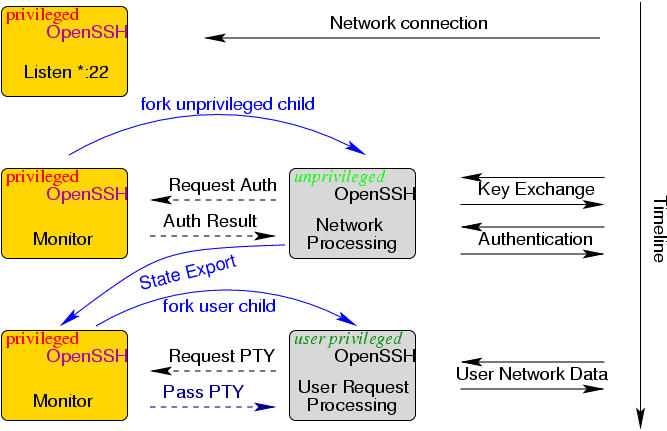
\includegraphics[width=\textwidth]{priv}
\end{figure}
\end{zhawframe}

\subsection{Forking}
\begin{zhawframe}
\begin{itemize}
\item<1-> Server spawns child to handle connection
\item<2-> \texttt{fork}(2)
\item<3-> Go: No support for forking
\item<4-> CGO fork fails
\item<5-> \texttt{syscall.ForkExec}

\onslide<6->$\rightarrow$ High level connection object gets corrupted
\item<7-> Create host application
\item<8-> Transfer \texttt{fd} as argument to child

\onslide<9->$\rightarrow$ Low level socket from \texttt{x/sys/unix} (x-package!)
\item<10-> Prospect: Implement proper privilege separation
\end{itemize}
\end{zhawframe}

\subsection{Login Accounting}
\begin{zhawframe}
\begin{itemize}
\item<1-> Not implemented, \textbf{but}
\item<2-> \texttt{utmpx} $\rightarrow$ \texttt{w}/\texttt{who}
\item<3-> PAM: \texttt{pam\_{}open\_{}session}(3)/\texttt{pam\_{}close\_{}session}(3)
\end{itemize}
\end{zhawframe}

\subsection{User Data Acquisition}
\begin{zhawframe}
\begin{itemize}
\item<1-> Home directory, shell, UID \& GID
\item<2-> Go standard library incomplete (misses shell information)
\item<3-> \texttt{/etc/passwd} (!)
\item<4-> CGO: \texttt{getpwnam}(2)/\texttt{getpwuid}(2)
\end{itemize}
\end{zhawframe}

\begin{frame}[fragile]{\insertsectionhead}{\insertsubsectionhead}
\lstset{
	style = basestyle,
	language = C,
}
\begin{lstlisting}
#include <sys/types.h>
#include <pwd.h>

struct passwd {
    char   *pw_name;       /* username */
    char   *pw_passwd;     /* user password */
    uid_t   pw_uid;        /* user ID */
    gid_t   pw_gid;        /* group ID */
    char   *pw_gecos;      /* user information */
    char   *pw_dir;        /* home directory */
    char   *pw_shell;      /* shell program */
};

struct passwd *getpwnam(const char *name);
struct passwd *getpwuid(uid_t uid);
\end{lstlisting}
\end{frame}

\subsection{Pseudoterminals}
\begin{zhawframe}
Shells expect to be connected to a TTY
\begin{figure}[ht]
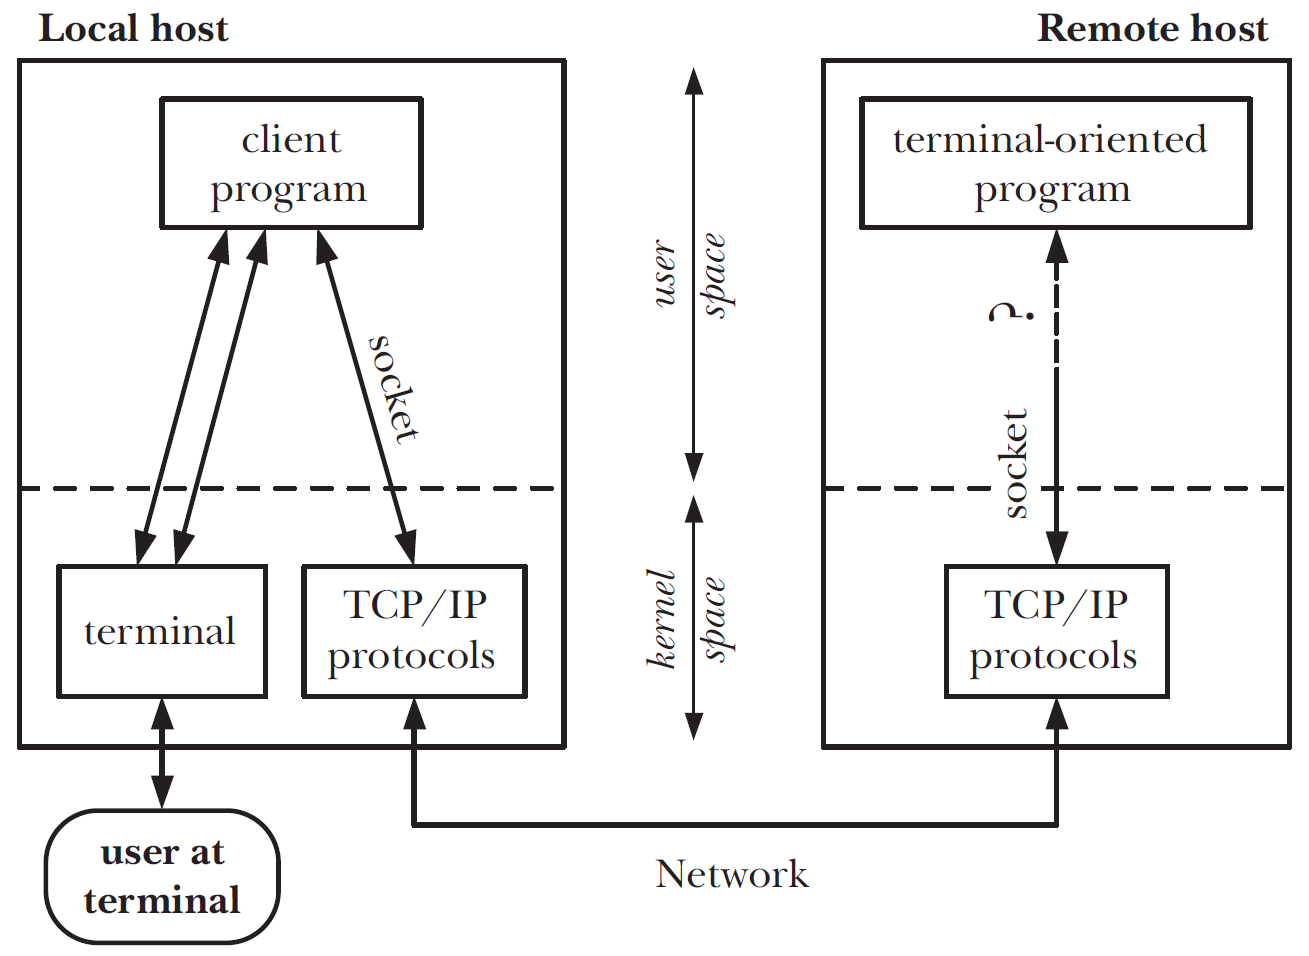
\includegraphics[width=0.8\textwidth]{PseudoterminalProblem}
\end{figure}
\end{zhawframe}

\begin{zhawframe}
PTY fakes being a TTY
\begin{figure}[ht]
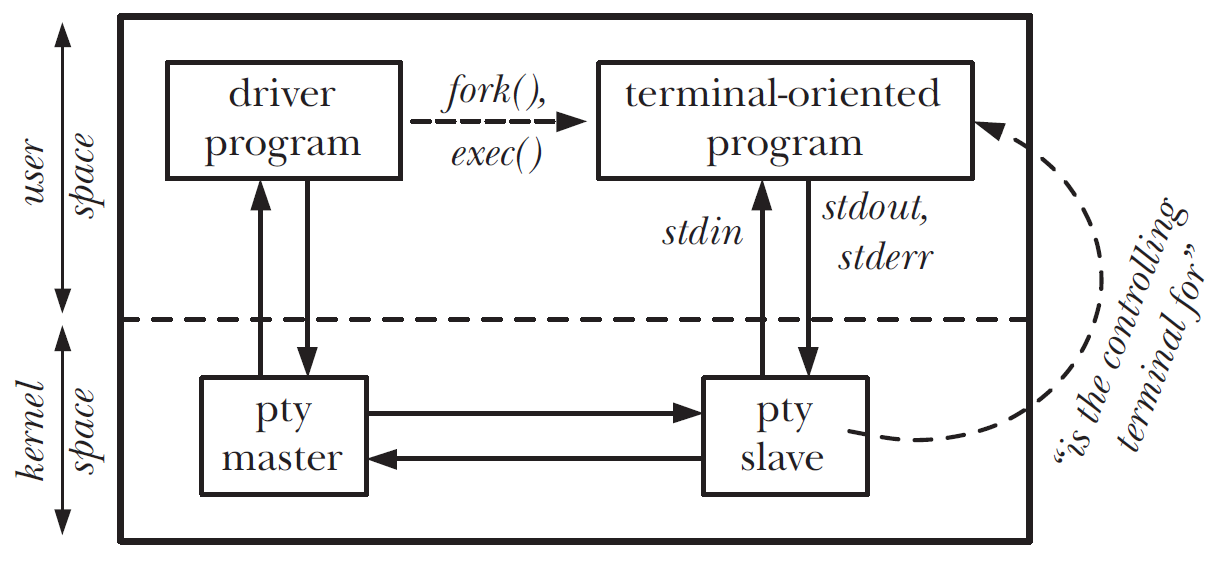
\includegraphics[width=0.94\textwidth]{Pseudoterminal}
\end{figure}
\end{zhawframe}

\begin{zhawframe}
Overview
\begin{figure}[ht]
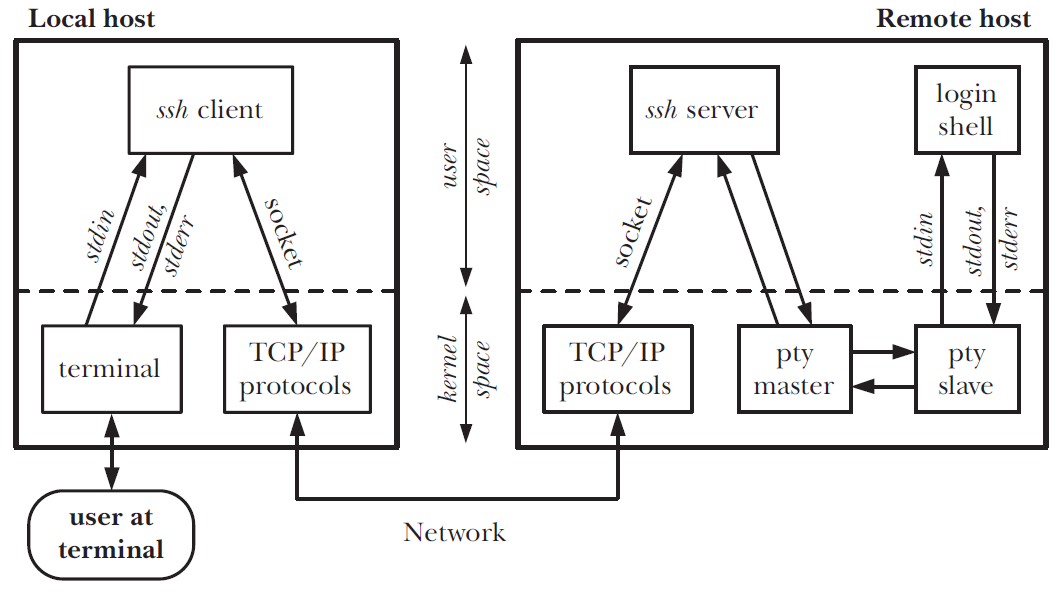
\includegraphics[width=0.85\textwidth]{PseudoterminalSSH}
\end{figure}
\end{zhawframe}

\begin{zhawframe}
\begin{itemize}
\item<1-> \texttt{istty}(3) on the connected \texttt{fd}s
\item<2-> \texttt{posix\_{}openpt("/dev/ptmx")}(3) $\rightarrow$ \texttt{grant\_{}pt}(3) $\rightarrow$ \texttt{unlockpt}(3) $\rightarrow$ \texttt{ptsname}(3)
\item<3-> Wrapper function in internal(!) package of the Go standard library \texttt{os/signal/internal/pty}
\end{itemize}
\end{zhawframe}

\begin{frame}[fragile]{\insertsectionhead}{\insertsubsectionhead}
\lstset{
	style = basestyle,
	language = Golang,
}
\begin{lstlisting}
// Open returns a master pty and the name of the linked slave tty.
func Open() (master *os.File, slave string, err error) {
    m, err := C.posix_openpt(C.O_RDWR)
    if err != nil {
        return nil, "", ptyError("posix_openpt", err)
    }
    if _, err := C.grantpt(m); err != nil {
        C.close(m)
        return nil, "", ptyError("grantpt", err)
    }
    if _, err := C.unlockpt(m); err != nil {
        C.close(m)
        return nil, "", ptyError("unlockpt", err)
    }
    slave = C.GoString(C.ptsname(m))
    return os.NewFile(uintptr(m), "pty-master"), slave, nil
}
\end{lstlisting}
\end{frame}

\subsection{Starting the Shell}
\begin{zhawframe}
\begin{itemize}
\item<1-> Shell requirements:
	\begin{itemize}
	\item user (UID \& GID) \& host name
	\item \texttt{TERM} env var (for \texttt{ncurses}(3X))
	\item window resolution (including \texttt{SIGWINCH})
	\item session leader (controlling terminal)
	\end{itemize}
\item<2-> Transfer of env vars (client $\leftrightarrow$ server)
\item<3-> Continuous transfer of \texttt{SIGWINCH} not implemented $\rightarrow$ prospects
\end{itemize}
\end{zhawframe}

\begin{frame}[fragile]{\insertsectionhead}{\insertsubsectionhead}
\lstset{
	style = basestyle,
	language = Golang,
}
\begin{lstlisting}
cmd := exec.Command(pwd.Shell, "--login")
cmd.SysProcAttr = &syscall.SysProcAttr{
    Setsid: true,
    //Setctty: true,
    Credential: &syscall.Credential{
        Uid: pwd.Uid,
        Gid: pwd.Gid,
    },
}
cmd.Env = userEnvs
\end{lstlisting}
\onslide<2-> Setting \texttt{CTTY} flag (for controlling terminal) fails $\rightarrow$ prospects
\end{frame}

\subsection{Terminal Mode}
\begin{zhawframe}
\begin{itemize}
\item<1-> Forward all keystrokes without interpretation (client-sside)
\item<2-> \texttt{cooked} mode $\rightarrow$ \texttt{raw} mode
\item<3-> x-package (!) \texttt{x/crypto/ssh/terminal}
\end{itemize}
\end{zhawframe}

\begin{frame}[fragile]{\insertsectionhead}{\insertsubsectionhead}
\lstset{
	style = basestyle,
	language = Golang,
}
\begin{lstlisting}
import "golang.org/x/crypto/ssh/terminal"
//...
oldState, err := terminal.MakeRaw(0)
if err != nil {
    panic(err)
}
defer terminal.Restore(0, oldState)
\end{lstlisting}
\end{frame}

\section{Evaluation}
\subsection{Performance}
\begin{zhawframe}
\begin{itemize}
\item<1-> client \textcolor{green!60!blue}{$\leftrightarrow$} server $\leftrightarrow$ ptm $\leftrightarrow$ pts $\leftrightarrow$ shell
\item<2-> \texttt{/dev/zero} $\rightarrow$ connection (client-side) $\rightarrow$ server $\rightarrow$ \texttt{pv -rabtW} $\rightarrow$ \texttt{/dev/null}
\item<3-> TLS vs no TLS
\end{itemize}
\onslide<4->
\begin{table}[ht]
\centering
\begin{tabular}{rcc}
Throughput with:				& TLS (size)	& no TLS (size)\\
								& MiB/s (GiB)	& MiB/s (GiB)\\\hline
Arch Linux (loopback) 			& 427 (25.1)	& 1177.6 (69.0)\\
WSL (loopback) 					& 69.7 (4.09)	& 116 (6.82)\\
Arch Linux to WSL (ethernet*) 	& 85.1 (4.99)	& 83.7 (4.91)
\end{tabular}
\end{table}
*: Netgear Switch \& Cat 5 ethernet cable
\end{zhawframe}

\subsection{Comparison to Telnet}
\begin{zhawframe}
\begin{itemize}
\item<1-> TLS vs plain text
\item<2-> Key auth vs only password auth
\end{itemize}
\end{zhawframe}

\subsection{Comparison to Berkeley \texttt{r}-commands}
\begin{zhawframe}
\begin{itemize}
\item<1-> Only \texttt{rlogin}(1) is considered (\texttt{rsh}(1))
\item<2-> TLS vs plain text
\item<3-> Key auth vs only password auth
\item<4-> Password auth: Both use \texttt{login}(1)
\end{itemize}
\end{zhawframe}

\subsection{Comparison to OpenSSH}
\begin{zhawframe}
\begin{itemize}
\item<1-> TLS vs own protocol
\item<2-> Privilege separation
\item<3-> Many additional features
\end{itemize}
\end{zhawframe}

\section{Conclusion}
\begin{zhawframe}
\begin{itemize}
\item<1-> Many problems encountered
\item<2-> Many new concepts learned
\item<3-> Mixed feelings
\end{itemize}
\end{zhawframe}

\section{End}
\begin{zhawframe}
Thank you for your attention!
\end{zhawframe}
\end{document}